\documentclass[a4paper,12pt]{article}
\usepackage[utf8x]{inputenc}
%\usepackage[spanish]{babel}
\usepackage{amsmath}
\usepackage{graphicx}
\setlength{\textheight}{235mm}
\setlength{\textwidth}{168mm}
\setlength{\oddsidemargin}{0pt}
\spanishdecimal{.}
\pagestyle{empty}

\begin{document}
\mbox{}\vspace*{-45mm}

{\centering
{\small\sc Escuela Técnica Superior de Ingenieros de Caminos, Canales y
Puertos (Madrid)}\\*[4mm]
{\Large\bf Método de los Elementos Finitos 23-24}\\*[4mm]
PRÁCTICA 3: Modelos de difusión \\*[4mm]
}

\vspace{3mm}


Se considera una chapa cuyas dimensiones y geometría son las indicadas
en la figura adjunta. Los lados de la chapa tienen condiciones de contorno 
correspondientes a temperaturas o flujos impuestos, cuyos valores
también están indicados en dicha figura. Los bordes en los que no se indica
el flujo o la temperatura impuesta se supone que están térmicamente aislados.
El coeficiente de conductividad térmica es $\lambda=1417.4$ W/(m$\cdot$C).

Se desea conocer la distribución de temperaturas y el flujo de calor en la
chapa realizando un modelo plano de elementos finitos. La discretización a efectuar corresponde a elementos cuadrados de cuatro
nodos de lado $0.5$ m.

Repetir el problema considerando dos materiales diferentes. El primero (parte superior con altura de 4m) tiene el mismo coeficiente de conductividad anterior; mientras que el resto de la parte inferior tiene $\lambda=932.5$ W/(m$\cdot$C). 

\vspace{3mm}


\begin{center}
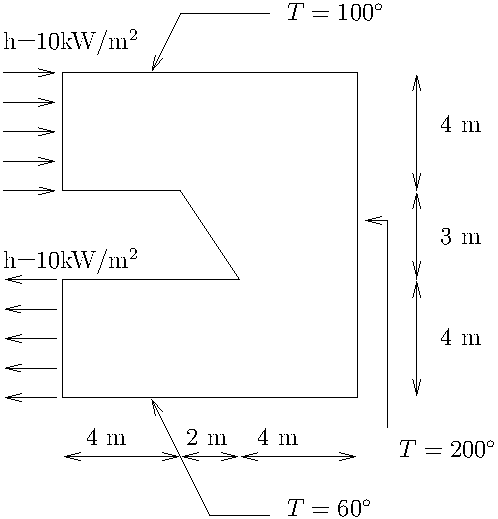
\includegraphics[width=0.55\textwidth]{practi4.pdf}
\end{center}

\end{document}

\end{document}
